\chapter{Approach} 
\label{chapter:approach}

Based on the background introduced in Chapter \ref{chapter:background}, a concept of 
a Convolutional Neural Network model, similar to the one proposed in \cite{DBLP:journals/corr/SantosXZ15}, 
but trained by means of Distant Supervision and improved by Multiple Instance Learning was developed.
An approach for implementation and evaluation on the selected datasets was introduced. 
First of all, the selected neural model 
should be implemented with one of the present programming libraries. The implementation 
should be proven to be correct via comparing the results achieved in the paper describing 
the model. Also, it is always useful to understand the underlying mechanism of the work of the 
network, thus different methods for interpretation of results might be utilised. The next main step is 
to make use of available Knowledge Bases and textual corpora by applying Distant Supervision. 
Afterwards, various methods for improvement of the achieved results can be implemented.
	
\section{Model description}
The model implemented for the research is a Convolutional Neural Network, that uses the idea 
of ranking for classification. It was implemented from scratch with 
Python, Tensorflow \footnote{https://www.tensorflow.org/} and Keras \footnote{https://keras.io/} 
libraries. As the idea of application of Deep Learning is to replace hand-crafted features for 
classifying relations Convolutional Neural Network model was selected instead of Recurrent Neural Network. 
Among all the models introduced for today the results of \cite{DBLP:journals/corr/SantosXZ15} 
showed up to be most impressive - so in \cite{nguyen2015combining} a combination of Recurrent 
Neural Networks and Convolutional Neural Networks gives the same results, in \cite{vu2016combining} 
a combination just slightly improves the result and a model based on various Natural Language Processing features 
\cite{gormley2015improved} also 
performs worse. And evaluation later showed that simple Recurrent Neural Network performed 
worse on one the testing datasets.

\subsection{Ranking convolutional neural network}
The model has the following structure:
\begin{enumerate}
\item \textbf{Words embeddings layer} The layer is responsible for transforming words of the input sentence to the embeddings. Every word $w_i$ of the sentence is transformed to a vector $r^{w_i}$. Every such vector is a row of an 
embedding matrix $W^{wrd}$ for some fixed-size vocabulary.
  Three types of word embeddings were used for experiments, in order to compare their effectiveness for the concrete task: 
   Word2Vec \cite{NIPS2013_5021}, GloVe \cite{pennington2014glove} and Swivel \cite{DBLP:journals/corr/ShazeerDEW16}. For each type 
  pre-trained versions were used if they were available on the internet. This was done because, as a rule, the quality of such versions is 
  comparatively high. Thus there is a variety of corpora that embeddings were trained 
  on. Information about the used embeddings can be found in the Table \ref{tab:emb}. The evaluation 
  showed that downloaded embeddings are more effective on average, thus proving the point 
  that accurate tuning of parameters and cross-validation on various tests of quality for word 
  embeddings can improve the result of the final model as well.
  
  \begin{table}
  \begin{center}
 \begin{tabular}{ | l | p{3.5cm} | p{3.5cm} | p{3.5cm} | }
    \hline
     & GloVe \footnote{Implementation and pre trained embeddings are from \url{http://nlp.stanford.edu/projects/glove/}} & Word2Vec \footnote{Implementation from \url{https://github.com/RaRe-Technologies/gensim}, pre trained embeddings from \url{https://drive.google.com/file/d/0B7XkCwpI5KDYNlNUTTlSS21pQmM/edit}} & Swivel \footnote{Implementation from \url{https://github.com/tensorflow/models/tree/master/swivel}} \\ \hline
    300 & downloaded, Wikipedia dump from 2014 and Gigaword 5 & downloaded, Google News corpus & trained locally, Wikipedia dump from 2016 \\ \hline
    400 & trained locally, Wikipedia dump from 2016 & trained locally, Wikipedia dump from 2016 & trained locally, Wikipedia dump from 2016 \\ \hline
    \end{tabular}
\caption[The word embeddings used for the experiments]{Summary of the embeddings used for the experiments.}
\label{tab:emb}
\end{center}
\end{table}

 The size of word embeddings $d^w$ is obtained by 4-fold validation experiments. Embeddings are modifiable during the training of the network, as it gives better results than 
 keeping them constant (proved empirically in \cite{DBLP:journals/corr/SantosXZ15}).
  
  \item \textbf{Distance embeddings layer} The layer is responsible for transforming distances between the words in the sentence 
  and marked named entities to the embedding vectors $wp_1$ and $wp_2$. Essentially, the vocabulary of these 
  embeddings is just numbers in the range $[p - l, p + l]$ where $l$ is the length of the 
  longest 
  sentence in the dataset and $p$ is some arbitrary big number, larger than the length of the 
  longest sentence. 
  The idea behind these embeddings is to point up the entities that are checked for the relation 
  to the network. This approach was introduced by \cite{zeng2014relation} and widely used 
  in many other works. There are also other ways of stressing the entities, for example 
  taking into account only part of the sentence between them, but according to the evaluation in  \cite{DBLP:journals/corr/SantosXZ15} position embeddings give the best results.
  The size of embeddings $d^{wpe}$ is obtained by 4-fold validation experiments. The grid for 
  search consisted of 30, 40, 50 and 70, as 70 was the embedding size used in the \cite{DBLP:journals/corr/SantosXZ15} and the intuition behind embeddings is that for smaller 
  vocabulary smaller dimension of embedding is needed. Embeddings are 
  initialized with random numbers uniformly distributed in {0,1} and learned during training of the 
  network.
  
  \item \textbf{Embeddings merge layer} The layer concatenates the word embedding $r^w$ and corresponding 
  distance embeddings (to the first named entity and to the second named entity) $wp_1$ and 
  $wp_2$ for every word $w$
  in the input sentence into one vector.
  
  \item \textbf{Convolutional layer} Convolution is applied to windows of three embedding vectors 
   with zero 
  padding, so the size of the input is not changed after the layer application.
  The number of filters $d^c$ is 1000 \cite{DBLP:journals/corr/SantosXZ15}, i.e. application of the filters 
  results into 1000 vectors of the same 
  length as the sentence, where each value in one vector is a feature value for a specific triplet of 
  words. The activation function applied after the filtering is \textit{tanh} \cite{DBLP:journals/corr/SantosXZ15}.
  
  \item \textbf{Global max pooling} The maximal value is found in the output of each filter. After this layer
  network has formed the universal representation of any sentence $r_x$ that is a real-valued vector in 
  1000-dimensional space. Application of global maximum allows not to take into account  
  different lengths of input sentences.
  
  \item \textbf{Scoring dense layer} In order to classify relations the closeness of a sentence 
  representation to real-valued vectors representing each of the relations that are learned during 
  the training process is 
  estimated. I.e. dot product of a sentence representation $r_x$ and each of the
  vectors that are called relation embeddings is calculated. The embedding that yields the maximal score is considered 
  to be the embedding of the relation described in the sentence. The output of the network is the 
  array of scores, for each of the classifiable relations. The scoring procedure is implemented
  as a dense layer without bias with weights matrix $W^{classes}$ consisting of the relations embeddings. The 
  weights are
  initialised randomly uniformly in the interval 
  $$\sqrt{\frac{6}{|C|+d^c}}$$
  where $C$ is a number of classifiable relations, $d^c$ is the length of sentence representation
  \cite{DBLP:journals/corr/SantosXZ15}.
  \end{enumerate}

	\begin{figure}
		\centering
		\includegraphics[width=180px]{chapter3_approach/images/ranking_cnn.png}
		\caption[Ranking Convolutional Neural Network]{Convolutional Neural Network for Relation Extraction with ranking \cite{DBLP:journals/corr/SantosXZ15}. The input to the network is a sentence with marked entities. The first transformation is performed by the matrix of word embeddings $W^{wrd}$ to obtain a dense representation of each word. Embeddings of the distances to the entities are obtained and concatenated together with the word embeddings. The second step is a convolution that results in $d^c$ values of filters for each window. Then global max pooling is applied to obtain the final representation of the sentence $r_x$ that is compared to each of the relation embeddings in the weight matrix $W^{classes}$.}
		\label{fig:ranking_cnn}
	\end{figure}

\subsection{Objective}
The objective function uses two of the resulting scores - one is the score, that was obtained for the 
correct relation according to the label of the example and the second score is one of the wrong 
relations scores. Ideally, according to \cite{DBLP:journals/corr/SantosXZ15} the second score 
should be the maximal score given to the wrong relations. 

Thus, objective calculation consists 
of the following steps:
\begin{itemize}
  \item Get the score to the correct relation from the array of scores and the correct label;
  \item Get the maximal score from the remaining wrong relations;
  \item Calculate the value of the loss according to the formula:
  $$L = log(1 + exp(\gamma(m^+ - s_{\theta}(x)_y^+))) + log(1 + exp(\gamma(m^- + s_{\theta}(x)_c^-)))$$
where $m^+$ is a margin for the right answer; $m^-$ is a margin for the wrong answers; $\gamma$ is a scaling factor; $s_{\theta}(x)_y^+$ is a score for the right class; $s_{\theta}(x)_c^-$ is a score for the wrong class. Margins and scaling factor are fixed numbers and their values are 
$m^+=2.5$, $m^-=0.5$, $\gamma=2$ as in \cite{DBLP:journals/corr/SantosXZ15}.
\end{itemize}

Intuitively, the minimisation of the loss leads to increasing the gap between the wrong score and 
the right
score by minimisation of the first one and maximisation of the second one. 

One special case for the objective function is behaviour with the class ''Other''. Class ''Other'' 
includes all the examples that are either describing relations that are not among main classes 
or do not describe any relation at all. According to \cite{DBLP:journals/corr/SantosXZ15} trying to make the network learn the 
embedding for the class ''Other'' leads to worse results, as it is very noisy and might also 
affect the results obtained for other classes. Therefore, when an example of ''Other'' class shown 
to the network objective function changes the first term (containing score for the right class) to 
zero. In this way the network is not learning anything about the ''Other'' class. During the 
recognition process example will be classified as ''Other'' only when the scores for all classes are 
negative. I.e. only when the network cannot classify example as any of desired classes it will reply 
that the class is unknown.

The loss also includes regularisation. L2 regularisation is applied on weights of the convolutional 
layer and the embeddings of the
relations (i.e. the weights of the last dense layer) with the regularisation rate 0.001 \cite{DBLP:journals/corr/SantosXZ15}.

A more common way for multi-class classification is an application of a softmax classifier after a 
dense layer to obtain the probability distribution. But according to evaluation experiments  in 
\cite{DBLP:journals/corr/SantosXZ15} ranking performs at least two percents better than softmax.

\subsection{Training}
Training is done by simple gradient descent with decaying learning rate. The learning rate is 
divided by the number of the epoch starting with the initial value of 0.025 \cite{DBLP:journals/corr/SantosXZ15}. Usually, the 
network almost stops learning after 10-20 epochs, because afterwards the 
gradient updates become very small and almost do not affect the result. 
The validation accuracy also stops improving and keeps fluctuating around the value reached before.

The training is organised by giving one sentence at a time, so the training data does not need 
to be padded to the same length. Epoch finishes after showing the network all sentences in the 
training set. After each epoch, the training set is shuffled randomly.

\section{Distant supervision}
As discussed in Chapter \ref{chapter:background}, Distant Supervision is used in order to overcome the problem of scarcity of training data for 
the neural network. In order to apply this concept, a Knowledge Base that contains desired relations 
is required along with large text corpus. An existing Knowledge Base is used for generating examples of relation 
mentions. This is achieved by aligning the entities from the Knowledge Base with the text corpus, either by simple string matching or more complex entity recognition solutions. Each sentence 
containing entity pair mention is considered to be labeled with the relation known for this pair 
from the Knowledge Base. So there are two assumptions made here:

\begin{enumerate}
  \item For every triple $(e_1, e_2, r)$ in a Knowledge Base every sentence containing mentions for 
  $e_1$ and $e_2$  express the relation $r$
  \item Every triple that is not in a Knowledge Base assumed to be a false example for relation, while 
   the reason might be in the incompleteness of knowledge.
\end{enumerate}

During the 
construction of distantly supervised training dataset, it is important to take into account the 
number of examples for each of the entity pairs and for each of the relations. It is very common 
that some of the pairs are much more often mentioned compared to other ones and the same 
is valid for the amounts of sentences for each relation because a Knowledge Base will not be 
balanced by the amount of triples for different relations.

There are different ways to evaluate the result of a 
distantly supervised model, one of them, for example, is to choose supervised dataset with the 
same relational classes and test the model. The main challenge in this approach is to find 
correspondence between existing labeled datasets and a public Knowledge Base. Empirically, it was 
found out that relations should be maximally similar, otherwise distant data will only introduce 
noise to the training process. Also, the corpora for aligning affect the quality of distantly 
supervised dataset a lot. \cite{riedel2010modeling} compared the amount of wrongly labeled 
examples when aligning Freebase to Wikipedia corpora and to New York Times news corpora. 
As it was expected Wikipedia has usually almost 10\% fewer mistakes. For example, if the 
relation ''Nationality'' is considered, it is quite possible that on news the country will be mentioned 
together with the person, but the exact relation of nationality is not described there. While 
Wikipedia will definitely contain sentences about the country of birth and residence of the person.

One more important point that should be taken into account when validating distantly supervised 
model with the existing testing dataset is that the underlying distribution behind supervised dataset 
most probably will differ from the distribution obtained from textual corpora 
\cite{craven1999constructing}. Same distribution in both training and testing datasets is one of the 
base assumptions for any supervised learner and it is extremely hard to control with distantly 
supervised datasets taking into account that even approximately same distribution in classes 
will not guarantee the same distribution of true underlying features of relations. 

In \cite{craven1999constructing} it is claimed that distantly supervised data improves precision 
but on the other hand following the results from \cite{riedel2010modeling} it also introduces 
noise, that definitely does not improve the precision. But on the other hand text corpora are 
very vast and definitely contain much more various syntactic constructions for defining 
specific relation, thus it might improve the recall of the model.

So several notes should be of importance for Distant Supervision:
\begin{enumerate}
  \item Exact correspondence between relations in Knowledge Base and desirable or described in 
  the supervised dataset;
  \item Appropriate textual corpora that contain information about desirable relations;
  \item Sufficient variety of syntactic constructions in testing set for adequate evaluation of the 
  results.
\end{enumerate}

\subsection{Multiple instance learning}
\label{subs:mil}
The assumption of the Distant Supervision is very imprecise as mostly sentences do not 
describe the relation that is stored in the Knowledge Base exactly. For solving this problem Multiple Instance Learning might be applied \cite{zeng2015distant}. 

This approach was first introduced for drugs classification - whether they are active or not 
\cite{dietterich1997solving}. The problem over there that every drug contains different 
molecules that are active or not, but only the activity of the drug is known. So in order to learn 
information about activity Multiple Instance Learning is performed - one label for several instances is 
known. One simple example can be seen in the Figure \ref{fig:mult-inst-learn}.

	\begin{figure}
		\centering
		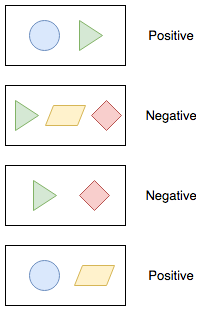
\includegraphics[width=150px]{chapter3_approach/images/mult-inst-learn.png}
		\caption[Multiple Instance Learning example]{Example of a dataset for Multiple Instance Learning. One of the hypotheses that can be suggested is that a blue circle makes the label positive, so this is the most important feature of a 'bag'.}
		\label{fig:mult-inst-learn}
	\end{figure}
	
In the application for Relation Extraction Multiple Instance Learning will mean, that we assume the
existence of at least one sentence containing the description of the relation from the 
Knowledge Base. One of the possibilities to construct bags is to unite the sentences with same entities mentions in one bag and give 
a corresponding label of the relation from the Knowledge Base. There are also different ways to train a neural
network with bags. The way from \cite{ramon2000multi} was chosen, i.e. the maximal score example should be chosen from the bag every 
time to fit the model. And all the bags are shuffled from epoch to epoch.

This approach is very naive and looses a lot of possibly useful information obtained by Distant Supervision,
 but it still can be used as an initial step for possible improvement of the approach.

\section{Interpretability evaluation}
In order to better understand the work of the neural network and the concept that was learned 
various insights could be used. Several of them were applied in this work.

\subsection{Representative trigrams}
\label{subs:repr-trigr}
According to \cite{DBLP:journals/corr/SantosXZ15} so-called representative trigrams can be  
extracted for classifiable relations. A representative trigram is a three words combination, that 
 characterises best (according to the network) one of the classes. They can be obtained from 
 the sentences of the dataset by measuring the value that each of trigrams in a sentence adds to the 
 correct class score. The value can be simply seen as a score that is obtained for the relational class, 
 if only one trigram of the sentence is seen. For better understanding of the way to obtain the 
 score for the trigram the Figure \ref{fig:repr-trigram} can be seen.
 
	\begin{figure}
		\centering
		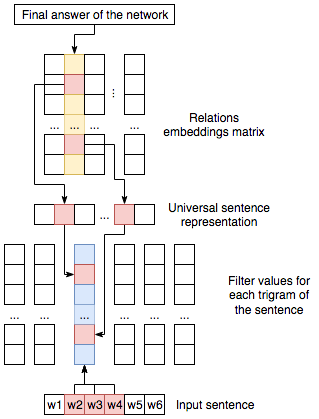
\includegraphics[width=200px]{chapter3_approach/images/repr-trigram.png}
		\caption[Schema of obtaining a trigram value]{Schematic view of tracing back the trigram, that made corresponding input to the final score of the relational class.}
		\label{fig:repr-trigram}
	\end{figure}

 This method is very similar to the one mentioned in 
 \cite{craven1999constructing} when the most valuable words were extracted in order to 
 have an insight into the concept learned by the model. For example, if "Origin" relation is learned, 
 one can expect to see the trigrams \textit{was born in, country of birth, was originated in}, etc.
 
\subsection{Semantic values}
\label{subs:sem-val}
The approach of \cite{DBLP:journals/corr/ZhangW15a} can be used to measure 
semantic values of each word in a sentence for classifying a relation between entities in the 
sentence. The idea of calculating is very close to finding representative trigrams, but in this case, the 
number of components of the resulting 1000-dimensional description of a sentence is taken 
as a characterising value. Thus, the initial trigram from the sentence was traced back for each component of a sentence description. The number of components of the sentence description 
vector traced back to the trigram is normalised by the dimension of the description vector (1000). 
This value is thought of as a semantic value for the central word of the trigram. There is a strong connection between 
representative trigrams and semantic values of the words of the sentence, as one can 
expect that the more characterising the words are, the larger their semantic value. For example, 
in the sentence 
\\
''$<e1>$George Walker Bush$</e1>$ was born on July 6, 1946, at Grace-New Haven Hospital (now Yale?New Haven Hospital) in New Haven, $<e2>$Connecticut$</e2>$, as the first child of George Herbert Walker Bush and his wife, the former Barbara Pierce." (\textit{Origin})
\\
one can expect large semantic values for words \textit{was born}.

\subsection{Scores distribution}
\label{subs:score-distr}
The way to understand better the answer given by the network is to display the scores distribution across the classes for a sentence. 
It can provide with information about how sure is the network about its answer that is usually 
an important characteristic of the machine learning model. Thus, big difference of scores 
between the right relation and wrong relation can show, that the network is sure and trained well 
enough for recognising this relation.

\section{Implementation details}
The network was implemented using Tensorflow, a Python library for tensor calculations and the 
high-level library Keras, that allows making the code more readable and understandable.

The experiments were run on NVIDIA Corporation GM200 [GeForce GTX TITAN X].

The structure of the network was visualised with Tensorboard \footnote{\url{https://www.tensorflow.org/get_started/summaries_and_tensorboard}} (Figure \ref{fig:tensorboard_vis}) that allows checking the correspondence to the desired structure. 

	\begin{sidewaysfigure}
		\centering
		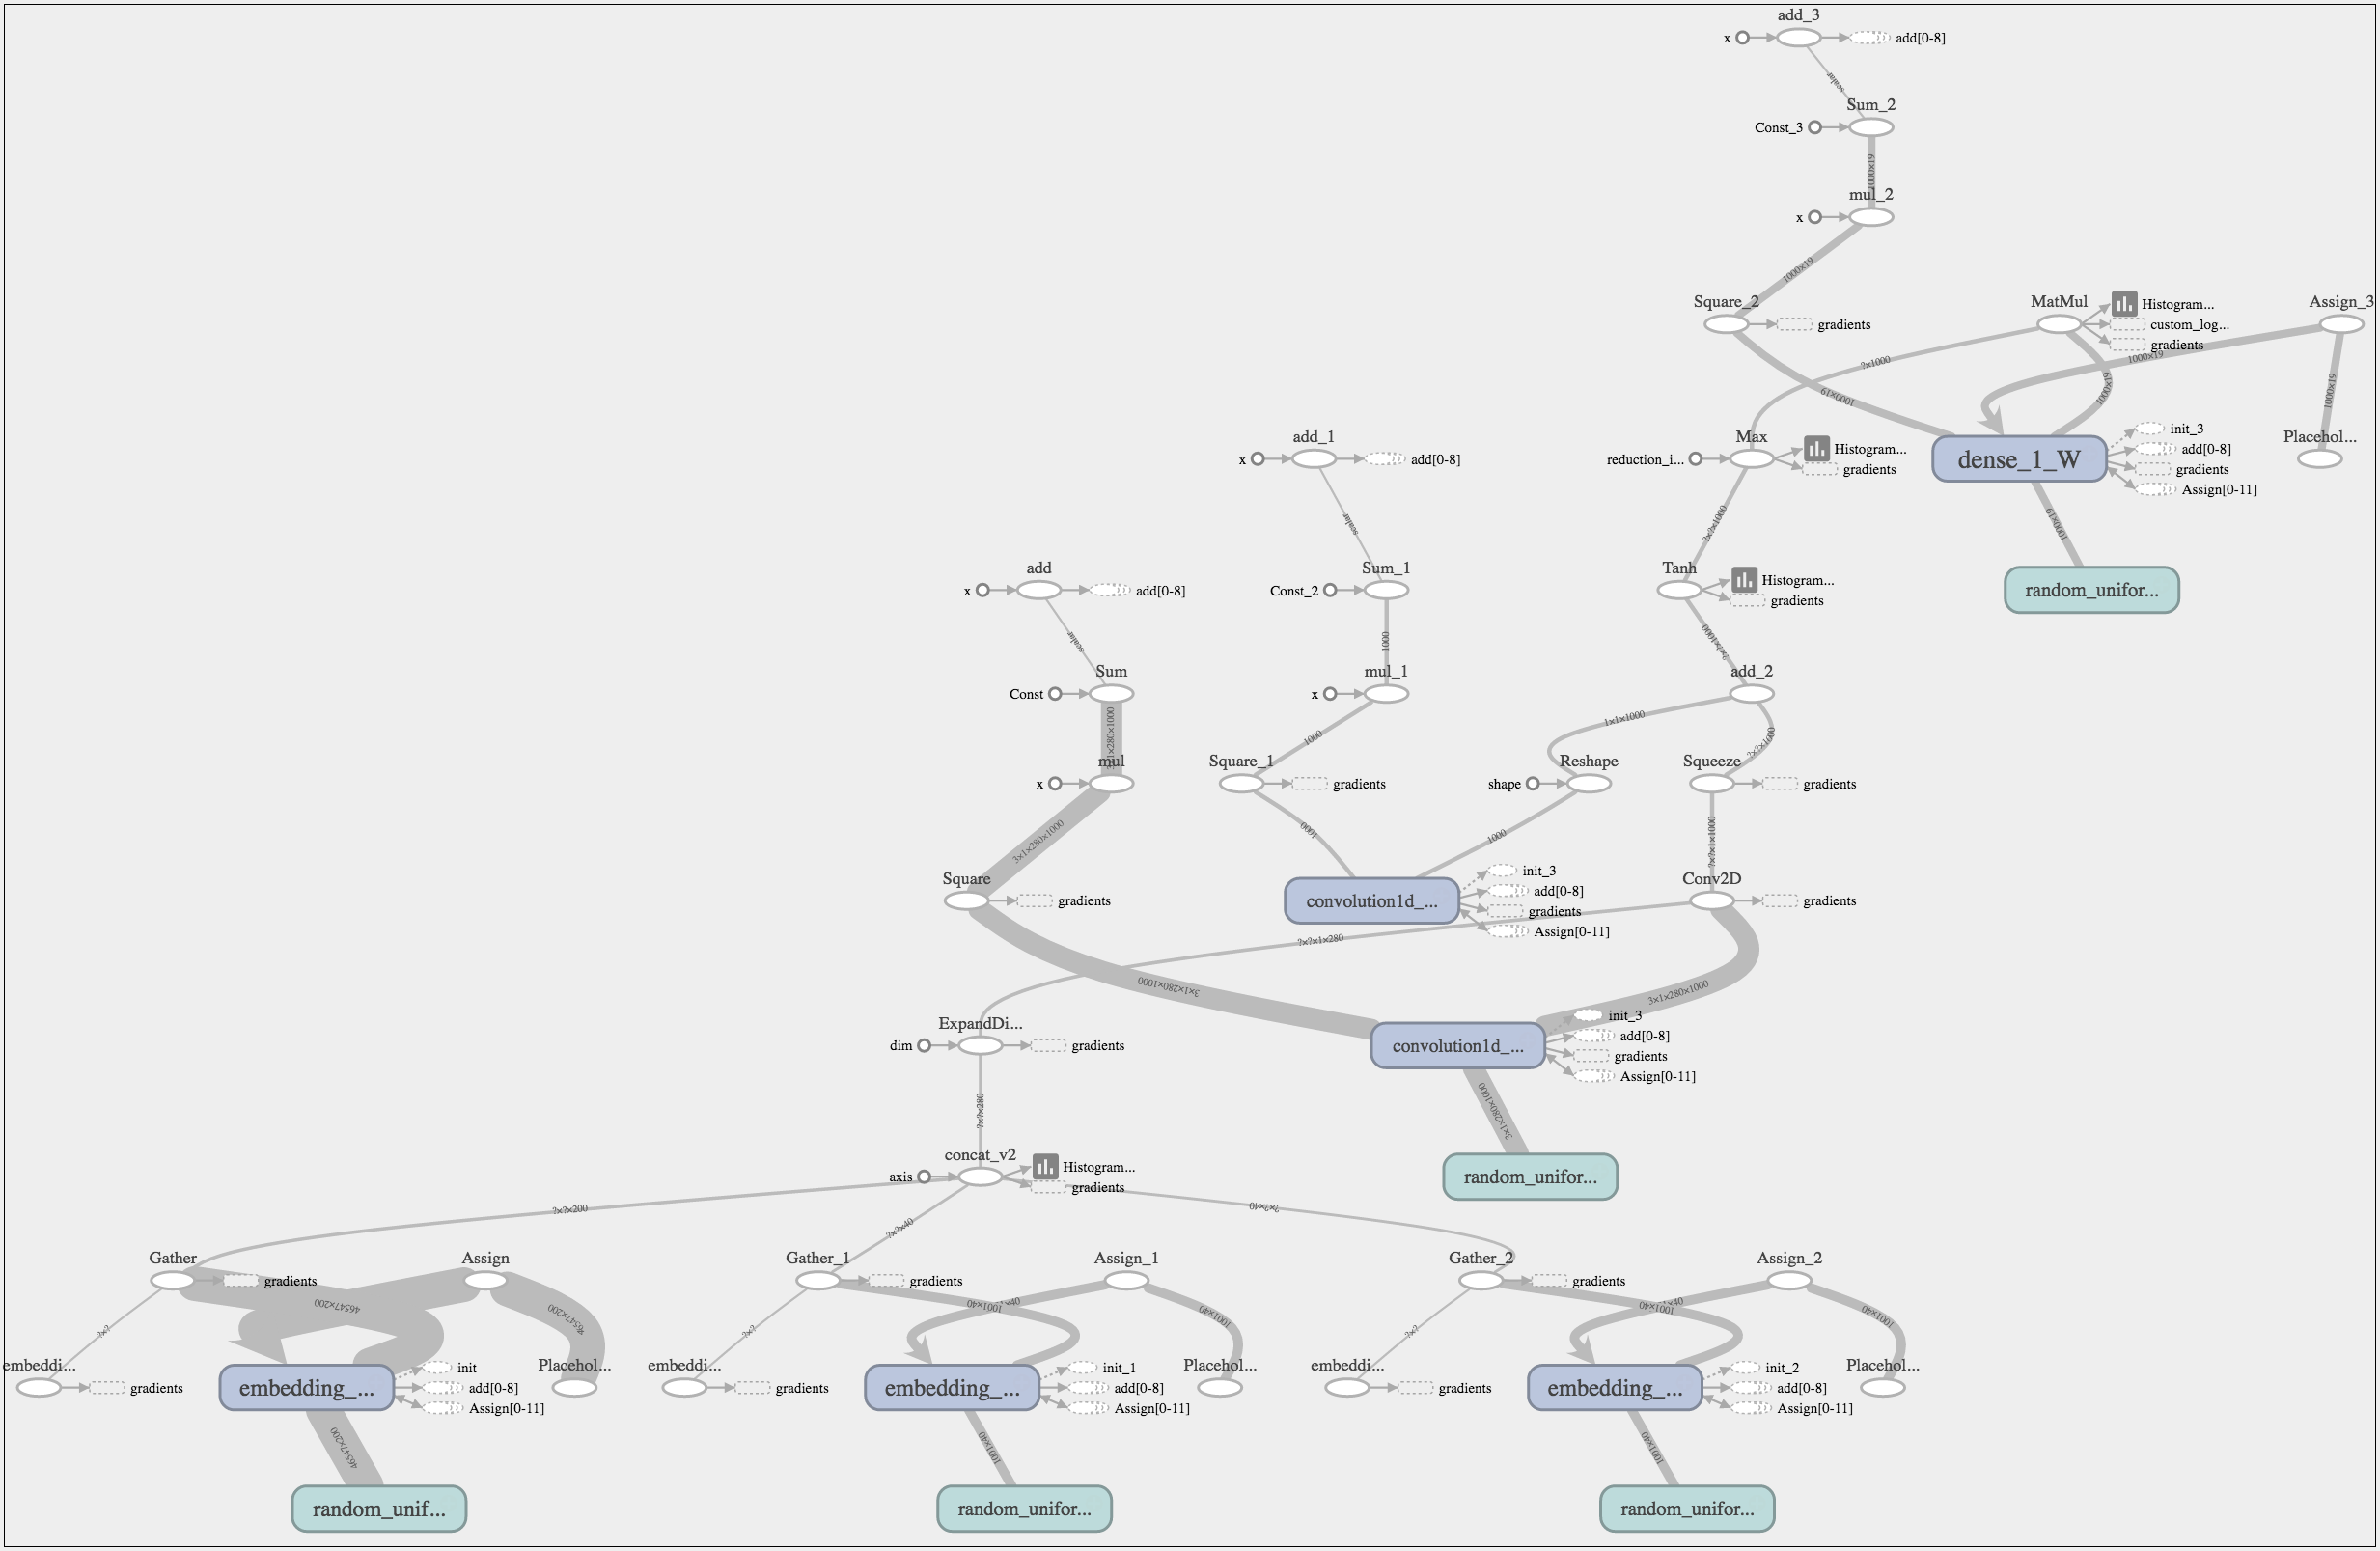
\includegraphics[width=\linewidth]{chapter3_approach/images/tensorboard_vis.png}
		\caption[Tensorboard visualisation of the network]{Screenshot from tensorboard visualisation of the implemented network. One can see three merging embedding layers in the bottom, that are followed by the convolutional layer. Then application of \textit{tanh} follows, after which \textit{Max} function and dense layer to get scores for each of the relations.}
		\label{fig:tensorboard_vis}
	\end{sidewaysfigure}

Following are several implementation details are listed:

\begin{itemize}
  \item
The input to the network is a single sentence with two marked named entities. Before application of convolution preprocessing 
is done. Preprocessing includes tokenisation and calculation of distances of each word to the first and second
named entities. Distance here is simply a number of words in between. It is negative when counted to the left and positive when counted to the right. For example, in the sentence ''The 
\textit{car} left the \textit{plant}.'' for token ''left'' distance to the first entity ''car'' is -1 and to the 
second entity ''plant'' is 2. The 
tokenisation was carried out by Penn Treebank tokeniser \footnote{\url{https://nlp.stanford.edu/nlp/javadoc/javanlp/edu/stanford/nlp/process/PTBTokenizer.html}} that is delivered by NLTK  python package \footnote{http://nltk.org}. The only modification that was applied on the text before tokenisation is down casing. The first layers of the network are embedding layers. They are applied in order to transfer tokens and distances to 
embedding vectors. Essentially, the task of an embedding layer is to substitute current token with 
its embedding, known beforehand. Usually, embeddings are stored in the form of the matrix, so 
the most straightforward implementation of an embedding layer is to find correspondence between a token and a row in the matrix. Thus all the tokens are transformed to indices, that 
represents the number of the row with embedding for this token. This functionality causes a problem for 
distance embeddings as distances might be negative when counted to the left of the token and 
cannot be used directly as indices in embeddings matrix.
In order to solve this issue, each distance was made 
positive by adding a large positive number $p$. As the maximal negative number cannot be 
larger by absolute value than the length of the longest sentence, it is easy to calculate this large 
number $p$. 

  \item In order to properly work with embeddings, the whole vocabulary of the embeddings 
  should be used in the matrix for the embeddings layer. But due to the Keras implementation of 
  the training, it becomes extremely slow with large sizes of the weights matrix. Also not all the 
  embeddings are supposed to change on each step. Therefore, it was decided to limit the vocabulary 
  only to the words that are there in the training and testing dataset. Also, Keras implements 
  dense updates for embedding layer, that extremely slows down the training, while Tensorflow 
  implementation uses sparse update. In order to get faster training native Tensorflow Gradient 
  Update was used \footnote{https://github.com/fchollet/keras/issues/4365}.
   \item Also, the vocabulary for the distances between words and entities was not described in the original paper. 
   It was chosen in the following way. Each distance was 
   summed with a large number $p$ (greater than the length of the 
  longest example) in order to make it positive and use as an index in embeddings 
  matrix. Thus, vocabulary consists of all the numbers from 0 to $2*p + 1$.
   \item As in the original paper sentence padding was not mentioned, the examples were decided 
  to give one-by-one and gradient step was performed after each sentence.
  \item The output of the network also was not described precisely. But as all the scores of all relations 
  are required to calculate the loss (one of the correct class and all others to find maximal wrong 
  value) it was decided to take the array of scores as the output and one hot encoded vector as a 
  label. Thus it is both possible to indicate the correct class score and maximal incorrect score in 
  the loss function calculation.
  \item Due to the form of the loss function, it can start overflow very fast (it uses exponent that is 
  an argument to logarithm and exponent can overflow already with rather small numbers). In the 
  first experiments 
  after first couple thousands of examples all the numbers started to become ''nan''. In order to fight this problem the work of TensorFlow was converted to ''float64'' regime, i.e. all the numbers 
  in tensors have this type.
\end{itemize}

